
% --------------------------------------------------------
% Tau
% LaTeX Template
% Version 2.4.2 (26/07/2024)
%
% Author: 
% Guillermo Jimenez (memo.notess1@gmail.com)
% 
% License:
% Creative Commons CC BY 4.0
% --------------------------------------------------------
%%%%%%%%%%%%%%%%%%%%%%%%%%%%%%%%%%%%%%%%%%%%%%%%%%%%%%%%%%%

\documentclass[9pt,a4paper,twoside]{tau-class/tau}
%\usepackage[english]{babel}


%% Spanish babel recomendation
% \usepackage[spanish,es-nodecimaldot,es-noindentfirst]{babel} 

%----------------------------------------------------------
% TITLE
%----------------------------------------------------------

\journalname{Example Template}
\title{\LaTeX\ class}

%----------------------------------------------------------
% AUTHORS, AFFILIATIONS AND PROFESSOR
%----------------------------------------------------------

\author[a,1]{Allen Issac}
%----------------------------------------------------------

\affil[a]{Affiliation of author one}
\affil[b]{Affiliation of author two}
\affil[c]{Affiliation of author three}

\professor{Professor/Authority or other information}

%----------------------------------------------------------
% FOOTER INFORMATION
%----------------------------------------------------------

\institution{College name}
\footinfo{\LaTeX\ Template}
\theday{July 26, 2024}
\leadauthor{Author last name et al.}
\course{Creative Commons CC BY 4.0}

%----------------------------------------------------------
% ABSTRACT AND KEYWORDS
%----------------------------------------------------------

\begin{abstract}    
    Welcome to tau ($\tau$) \LaTeX\ class designed especially for your lab reports or academic articles. In this example template, we will guide you through the process of using and customizing this class to your needs. For more information of this class check out the appendix section. There, you will find codes that define key aspects of the template, allowing you to explore and modify them.
\end{abstract}

%----------------------------------------------------------

\keywords{\LaTeX\ class, lab report, academic article, tau class}

%----------------------------------------------------------

\begin{document}
		
    \maketitle 
    \thispagestyle{firststyle} \tauabstract 
    \tableofcontents
    \linenumbers 
    
%----------------------------------------------------------

\section{Introduction}

    \taustart{W}elcome to \textit{tau class} for preparing your lab reports or academic articles. Throughout this guide, we will show you how to use this template and how to make modifications to this class. 
	
    This class includes the following files placed in the ‘tau-class’ folder: tau.cls, tauenvs.sty, taubabel.sty and README.md. Also, a main.tex, tau.bib and some examples. 

\section{Title}

    The \verb*|\maketitle| command generates the title and author information section, including the professor name and affiliations. The title can be modified in tau-class/tau.cls/title style section. 
	
    By default, \textit{tau class} shows the title on the left. However, you can change \verb*|\raggedright| to \verb*|\centering| in \verb*|\titlepos| to move the title to the center or, modify it to your own preferences.
	
    In addition to the \verb|\title| command, a new command named \verb|\journalname| has been added to include more information. 
	
    If you do not need this command, you can undefined it and the content will be adjusted automatically.
	
\section{Abstract}

    The abstract and keywords are defined using the \verb*|\keywords| and \verb*|\begin{abstract} \end{abstract}| commands respectively. For the abstract to appear, make sure the \verb|\tauabstract| command is always included after the beginning of the document.
    
    If the keywords are not declared in the preamble, the content will be adjusted automatically.
    
\section{Document style options}

    \subsection{Tau start}
	
        We included the \verb|\taustart{}| command, which provides a personalized lettrine for the beginning of a paragraph.

    \subsection{Line numbering}
	
        By implementing the \textit{lineno} package, the line numbering of the document can be placed with the command \verb|\linenumbers|. 
		
        I recommend placing the command after the abstract and table of contents for a better appearance (comment or delete if not required).
		
    \subsection{Table of contents}
	
        The \textit{tau class} provides a customized design for the table of contents. Each level of the ToC provides a preview of the content and its location in the document. 
		
\section{Figures and tables}

    \subsection{Figures}
		
%	Fig. \ref{fig:figure} shows an example figure.
		
	\begin{figure}[H]
		\centering
		
\includegraphics[width=0.75\columnwidth]{arch.png}
%		\caption{Example figure obtained from PGFPlots \cite{PFGPlots}.}
		\label{fig:figure}
	\end{figure}
		
%        Fig. \ref{fig:examplefloat} shows an example of two figures that covers the width of the page. It can be placed at the top or bottom of the page. The space between the figures can also be changed using the \verb|\hspace{Xpt}| command.
		
        \begin{figure*}[tp] % t for position at the top of the current page; b for position at the bottom; p for new page
		\centering
		  \begin{subfigure}[b]{0.38\linewidth} % Fig (a)
			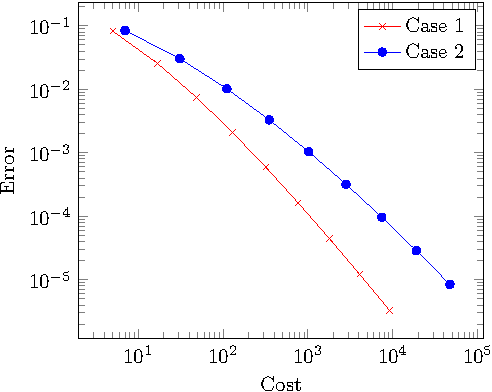
\includegraphics[width=\linewidth]{Example2.pdf}
			\caption{Example left figure.}
			\label{fig:figa}
		\end{subfigure}
			\hspace{20pt}   % Space between the figures
		\begin{subfigure}[b]{0.375\linewidth} % Fig (b)
			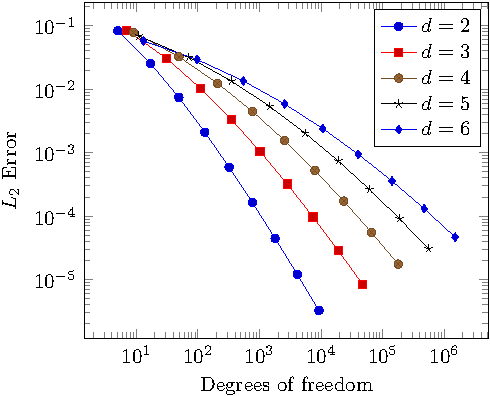
\includegraphics[width=\linewidth]{Example3.pdf}
			\caption{Example right figure.}
			\label{fig:figb}
		\end{subfigure}
%		\caption{Example figure that covers the width of the page obtained from PGFPlots \cite{PFGPlots}.}
		\label{fig:examplefloat}
	\end{figure*}
	
    \subsection{Tables}
	
%        Table \ref{tab:table} shows an example table. The \verb|\tabletext{}| is used to add notes to tables easily. 
		
	\begin{table}[H]
		\centering
		\caption{Small example table.}
		\label{tab:table}
		\begin{tabular}{cc}
			\toprule
			\textbf{Column 1} & \textbf{Column 2} \\
			\midrule
			Data 1 & Data 2 \\
			Data 3 & Data 4 \\
			\bottomrule
		\end{tabular}
			
            \tabletext{Note: I'm a table text for additional information.}
			
	\end{table}
		
\section{Tau packages}

    \subsection{Tauenvs}
	
        This template has its own environment package \textit{tauenvs.sty} designed to enhance the presentation of the document. Among these custom environments are \textit{tauenv}, \textit{info} and \textit{note}.
		
        There are two environments which have a predefined title. These can be included by the command \verb|\begin{note}| and \verb|\begin{info}|. All the environments have the same style.
			
        An example using the tau environment is shown below.
		
	\begin{tauenv}[frametitle=Environment with custom title]
            This is an example of the custom title environment. To add a title type \verb|[frametitle=Your title]| next to the beginning of the environment (as shown in this example).
	\end{tauenv}
		
        Tauenv is the only environment that you can customize its title. On the other hand, info and note adapt their title to Spanish automatically when this language package is defined.
		
    \subsection{Taubabel}

        In this new version, we have included a package called \textit{taubabel}, which have all the commands that automatically translate from English to Spanish when this language package is defined. 
        
        By default, tau displays its content in English. However, at the beginning of the document you will find a recommendation when writing in Spanish. 
		
        \textit{Note:} You may modify this package if you want to use other language than English or Spanish. This will make easier to translate the document without having to modify the class document.
		
\section{Equation}

%    Equation \ref{ec:equation}, shows the Schrödinger equation as an example. 
	\begin{equation} \label{ec:equation}
		\frac{\hbar^2}{2m}\nabla^2\Psi + V(\mathbf{r})\Psi = -i\hbar \frac{\partial\Psi}{\partial t}
	\end{equation} 
    The \textit{amssymb} package was not necessary to include, because stix2 font incorporates mathematical symbols for writing quality equations. In case you choose another font, uncomment this package in tau-class/tau.cls/math packages.
	
    If you want to change the values that adjust the spacing above and below the equations, play with \verb|\setlength{\eqskip}{8pt}| value until the preferred spacing is set.
	
\section{Adding codes}
	
    This class\footnote{Hello there! I am a footnote :)} includes the \textit{listings} package, which offers customized features for adding codes in \LaTeX\ documents specifically for C, C++, \LaTeX\ and Matlab. 
	
    You can customize the format in tau-class/tau.cls/listings style.
	
        \nolinenumbers
            \lstinputlisting[caption=Example of Matlab code., language=Matlab,label=code]{example.m}
	\linenumbers
	
    If line numbering is defined at the beginning of the document, I recommend placing the command \verb|\nolinenumbers| at the start and \verb|\linenumbers| at the end of the code. 
	
    This will temporarily remove line numbering and the code will look better as shown in Code \ref{code}.
	
\section{References}

    The default formatting for references follows the IEEE style. You can modify the style of your references, for that, go to tau-class/tau.cls/biblatex. See appendix for more information.
	
\section{Appendix}

    \subsection{Alternative title}

        You can make the following modification in tau-class/tau.cls/title preferences section to change the position of the title.

\nolinenumbers
\begin{lstlisting}[language=TeX, caption=Alternative title.]
\newcommand{\titlepos}{\centering}
\end{lstlisting}
\linenumbers

	This will move the title to the center. 

    \subsection{Info environment}

        An example of the info environment declared in the ‘tauenvs.sty’ package is shown below. Remember that \textit{info} and \textit{note} are the only packages that translate their title (English or Spanish).
		
%	\begin{info}
%		Small example of info environment.
%	\end{info}

    \subsection{Equation skip value}

        With the \verb|\eqskip| command you can change the spacing for equations. The default \textit{eqskip} value is 8pt.

\nolinenumbers
\begin{lstlisting}[language=TeX, caption=Equation skip code.]
\newlength{\eqskip}\setlength{\eqskip}{8pt}
	\expandafter\def\expandafter\normalsize\expandafter{%
		\normalsize%
		\setlength\abovedisplayskip{\eqskip}%
		\setlength\belowdisplayskip{\eqskip}%
		\setlength\abovedisplayshortskip{\eqskip-\baselineskip}%
		\setlength\belowdisplayshortskip{\eqskip}%
	}
\end{lstlisting}
\linenumbers
		
    \subsection{References}
		
        In case you require another reference style, you can go to tau-class/tau.cls/biblatex and modify the following.
		
\nolinenumbers

%----------------------------------------------------------

\end{document}
